\section{Force and Momentum Conservation\footnote{
1990-93 Dept. of Physics and Astronomy, Dickinson College. Supported by FIPSE
(U.S. Dept. of Ed.) and NSF. Portions of this material may have been modified
locally and may not have been classroom tested at Dickinson College.
}}

Name \rule{2.0in}{0.1pt}\hfill{}Section \rule{1.0in}{0.1pt}\hfill{}Date \rule{1.0in}{0.1pt}

\textbf{Objectives} 

\begin{itemize}
\item To understand the definition of momentum and its vector nature and its relationship
to Newton's second law. 
\item To explain how forces act over time when an object undergoes a collision. 
\item To use Newton's second law to develop a mathematical equation relating impulse
and momentum change for any object experiencing a force.
\item To formulate the Law of Conservation of Momentum as a theoretical consequence
of Newton's laws and to test it experimentally.
\end{itemize}
\textbf{Overview }

In the next few units we will explore the forces of interaction between two
or more objects and study the changes in motion that result from these interactions.
We are especially interested in studying collisions and explosions in which
interactions take place in fractions of a second or less. Early investigators
spent a considerable amount of time trying to observe collisions and explosions,
but they encountered difficulties. This is not surprising, since the observation
of the details of such phenomena requires the use of instrumentation that was
not yet invented (such as the high speed camera). However, the principles of
the outcomes of collisions were well understood by the late seventeenth century,
when several leading European scientists (including Sir Isaac Newton) developed
the concept of ``quantity of motion'' 
to describe both elastic collisions (in which
objects bounce off each other) and inelastic collisions (in which objects stick
together). These days we use the word momentum rather than motion in describing
collisions and explosions.

We will begin our study of collisions by exploring the relationship between
the forces experienced by an object and its momentum change. It can be shown
mathematically from Newton's laws and experimentally from our own observations
that the integral of force experienced by an object over time is equal to its
change in momentum. This time-integral of force is defined as a special quantity
called impulse, and the statement of equality between impulse and momentum change
is known as the impulse-momentum theorem.

\textbf{Apparatus} 

\begin{center}
\begin{tabular}{|p{1.5in}|p{1.5in}|p{1.75in}|} \hline
Dynamics carts (4) and track                         & 2 force probes (force sensors) & \textit{Science Workshop 750 Interface} \\ \hline
Graphing and curve fitting software (\textit{Excel}) & Circular bubble level          & \textit{DataStudio} software (Two Force Probes application) \\ \hline
Weights                                              &                                &                                            \\ \hline
\end{tabular}
\end{center}


\textbf{Defining Momentum }

In this session we are going to develop the concept of momentum to predict the
outcome of collisions. But you don't officially know what momentum is because
we haven't defined it yet. Lets start by predicting what will happen as a result
of a simple one-dimensional collision. This should help you figure out how to
define momentum to enable you to describe collisions in mathematical terms.

\vspace{0.3cm}
{\par\centering 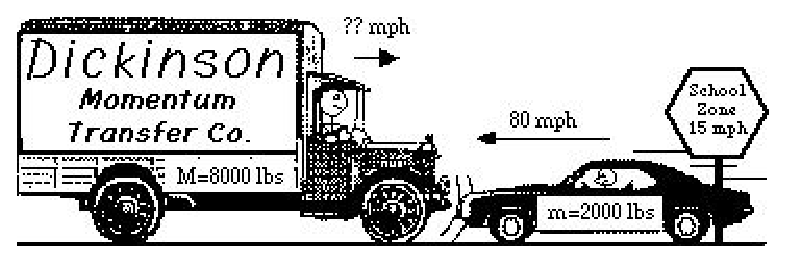
\includegraphics{momentum/momentum_fig1.eps} \par}
\vspace{0.3cm}

It's early fall and you are driving along a two lane highway in a rented moving
van. It is full of all of your possessions so you and the loaded truck were
weighed in at 8000 lbs. You have just slowed down to 15 MPH because you're in
a school zone. It's a good thing you thought to do that because a group of first
graders is just starting to cross the road. Just as you pass the children you
see a 2000 lb sports car in the oncoming lane heading straight for the children
at about 80 MPH. What a fool the driver is! A desperate thought crosses your
mind. You figure that you just have time to swing into the oncoming lane and
speed up a bit before making a head-on collision with the sports car. You want
your truck and the sports car to crumple into a heap that sticks together and
doesn't move. Can you save the children or is this just a suicidal act? For
simulated observations of this situation you can use two carts of different
masses set up to stick together in trial collisions. 

\textbf{Activity \stepcounter{activity}\arabic{activity}: Can You Stop the Car?} 

(a) Predict how fast you would have to be going to completely stop the sports
car. Explain the reasons for your prediction.
\vspace{20mm}

(b) Try some head on collisions with the carts of different masses and without
a force sensor attached to simulate
the event. Describe some of your observations. What happens when the less massive
cart is moving much faster than the more massive cart? Much slower? At about
the same speed?
\vspace{20mm}

(c) Based on your intuitive answers in parts (a) and (b) and your observations,
what mathematical definition might you use to describe the momentum (or motion)
you would need to stop an oncoming vehicle traveling with a known mass and velocity?
\vspace{20mm}

Just to double check your reasoning, you should have come to the conclusion
that momentum is defined by the vector equation
\[
{\bf p}=m{\bf v}.\]

\newpage


\textbf{Expressing Newton's Second Law Using Momentum }

Originally Newton did not use the concept of acceleration or velocity in his
laws. Instead he used the term ``motion,'' which he defined
as the product of mass and velocity (a quantity we now call momentum). Let's
examine a translation from Latin of Newton's first two laws (with some parenthetical
changes for clarity).

\textit{Newton's First Two Laws of Motion}

\begin{enumerate}
\item \textit{Every body continues in its state of rest, or of uniform motion in a
right line, unless it is compelled to change that state by forces impressed
on it. }
\item \textit{The (rate of) change of motion is proportional to the motive force impressed:
and is made in the direction in which that force is impressed.}
\end{enumerate}
The more familiar contemporary statement of the second law is that the net force
on an object is the product of its mass and its acceleration where the direction
of the force and of the resulting acceleration are the same. Newton's statement
of the law and the more modern statement are mathematically equivalent, as you
will show.

\textbf{Activity \stepcounter{activity}\arabic{activity}: Re-expressing Newton's Second Law}\actlabel{secondLaw}

(a) Write down the contemporary mathematical expression for Newton's second
law relating net force to mass and acceleration. Please use vector signs and
a summation sign where appropriate.
\vspace{10mm}

(b) Write down the definition of instantaneous acceleration in terms of the
rate of change of velocity. Again, use vector signs.
\vspace{10mm}

(c) If an object has a changing velocity and a constant
mass then \( m\frac{d{\bf v}}{dt}=\frac{d\left( m{\bf v}\right) }{dt} \).
Explain.
\vspace{20mm}

(d) Show that \( \sum {\bf F}=m{\bf a}=\frac{d{\bf p}}{dt} \).
\vspace{20mm}

(e) Explain in detail why Newton's statement of the second law and the mathematical
expression \( \sum {\bf F}=\frac{d{\bf p}}{dt} \) are
two representations of the same statement, i.e., are logically equivalent.
\vspace{20mm}

%--------------------------------------------------------------------

\textbf{Predicting Interaction Forces between Objects} 

We recently focused our attention on the change in momentum that an object undergoes
when it experiences a force that is extended over time (even if that time is
very short!). Since interactions like collisions and explosions never involve
just one object, we would like to turn our attention to the mutual forces of
interaction between two or more objects. As usual, you will be asked to make
some predictions about interaction forces and then be given the opportunity
to test these predictions. 

\textbf{Activity \stepcounter{activity}\arabic{activity}: Predicting Interaction Forces} 

(a) Suppose the masses of two objects are the same and that the objects are
moving toward each other at the same speed so that
\[
m_{1}=m_{2}\quad \mbox{and}\quad {{\bf v}_{1}}=-{{\bf v}_{2}}\]


\vspace{0.3cm}
{\par\centering 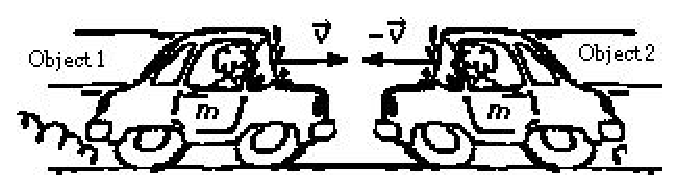
\includegraphics{momentum/newtons_laws_fig1.eps} \par}
\vspace{0.3cm}

Predict the relative magnitudes of the forces between object 1 and object 2.
Place a check next to your prediction! 

\rule{0.5in}{0.1pt} Object 1 exerts more force on object 2. 

\rule{0.5in}{0.1pt} The objects exert the same force on each other. 

\rule{0.5in}{0.1pt} Object 2 exerts more force on object 1.

(c) Suppose the mass of object 1 is much less than that of object 2 and that
it is pushing object 2 that has a dead motor so that both objects move in the
same direction at speed v.
\[
m_{1}\ll m_{2}\quad \mbox{and}\quad {{\bf v}_{1}}={{\bf v}_{2}}\]


\vspace{0.3cm}
{\par\centering 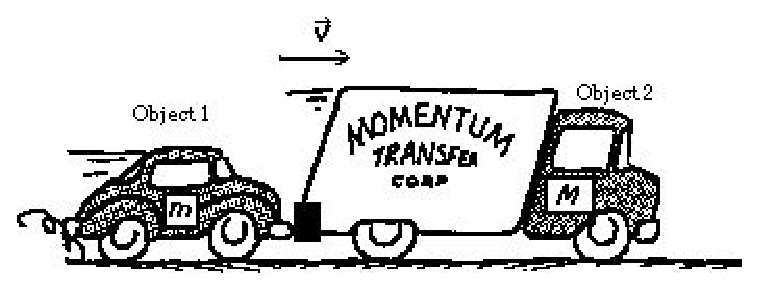
\includegraphics{momentum/newtons_laws_fig3.eps} \par}
\vspace{0.3cm}

Predict the relative magnitudes of the forces between object 1 and object 2.
Place a check next to your prediction. 

\rule{0.5in}{0.1pt} Object 1 exerts more force on object 2. 

\rule{0.5in}{0.1pt} The objects exert the same force on each other. 

\rule{0.5in}{0.1pt} Object 2 exerts more force on object 1.

\newpage

(d) Suppose the mass of object 1 is greater than that of object 2 and that the
objects are moving toward each other at the same speed so that
\[
m_{1}>m_{2}\quad \mbox{and}\quad {{\bf v}_{1}}=-{{\bf v}_{2}}\]


\vspace{0.3cm}
{\par\centering 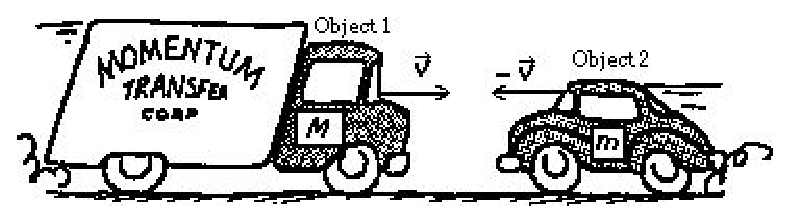
\includegraphics{momentum/newtons_laws_fig4.eps} \par}
\vspace{0.3cm}

Predict the relative magnitudes of the forces between object 1 and object 2.
Place a check next to your prediction. 

\rule{0.5in}{0.1pt} Object 1 exerts more force on object 2. 

\rule{0.5in}{0.1pt} The objects exert the same force on each other.

\rule{0.5in}{0.1pt} Object 2 exerts more force on object 1.

(e) Suppose the mass of object 1 is greater than that of object 2 and that object
2 is moving in the same direction as object 1 but not quite as fast so that
\[
m_{1}>m_{2}\quad \mbox{and}\quad {{\bf v}_{1}}>{{\bf v}_{2}}\]


\vspace{0.3cm}
{\par\centering 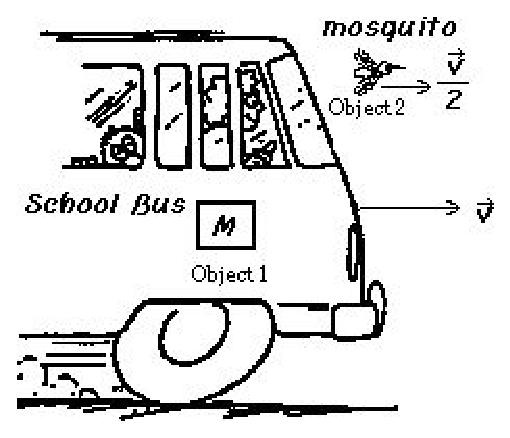
\includegraphics{momentum/newtons_laws_fig5.eps} \par}
\vspace{0.3cm}

Predict the relative magnitudes of the forces between object 1 and object 2.
Place a check next to your prediction. 

\rule{0.5in}{0.1pt} Object 1 exerts more force on object 2. 

\rule{0.5in}{0.1pt} The objects exert the same force on each other. 

\rule{0.5in}{0.1pt} Object 2 exerts more force on object 1.

\newpage

(g) Provide a summary of your predictions. What are the circumstances under
which you predict that one object will exert more force on another object?
\vspace{30mm}

\textbf{Measuring Mutual Forces of Interaction }

In order to test the predictions you made in the last activity you can study
gentle collisions between two force probes attached to carts. You can strap
additional masses to one of the carts to increase its total mass so it has significantly
more mass than the other. If a compression spring is available you can set up
an ``explosion'' between the two carts by compressing the spring
between the force probes on each cart and letting it go. You can make and display the 
force measurements with the \textbf{Two Force Probes} application 
in the \textbf{131 Workshop} submenu. 
You can also determine the areas under the force vs. time graphs to find the 
impulses experienced by the carts during the collisions. 
See \textbf{Appendix B Introduction to DataStudio}
for instructions on finding the area under a curve.

\textbf{Activity \stepcounter{activity}\arabic{activity}: Measuring Collision Forces }

(a) Use the two carts with force sensors 
to explore various situations that correspond to the predictions
you made about mutual forces. 
Your goal is to find out under what circumstances
one object exerts more force on another object. Describe what you did in the
space below and attach a printout of at least one of your graphs of force 1
vs. time and force 2 vs. time.
\vspace{40mm}

(b) What can you conclude about forces of interactions during collisions? Are there any circumstances 
under which one object experiences a different magnitude of force
than another during a collision? How do the magnitudes and directions of the
forces compare on a moment by moment basis in each case? 
Were the predictions you made correct?
If not, explain why.

\vspace{30mm}

(c) Do your conclusions have anything to do with Newton's third law?
\vspace{20mm}

\newpage

(d) How does the vector force due to object 1 acting on object 2 compare to
the force of object 2 acting on object 1 in each case? Are they the same in
magnitude or different? Do they have the same sign or a different sign? 
%Remember \( {\bf I}=\int _{t_{i}}^{t_{f}}{\bf F}\,dt \).
\vspace{30mm}

\textbf{Newton's Laws and Momentum Conservation} 

In your investigations of interaction forces, you should have found that the
forces between two objects are equal in magnitude and opposite in sign on a
moment by moment basis for all the interactions you studied. This is of course
a testimonial to the seemingly universal applicability of Newton's third law
to interactions between ordinary masses. You can combine the findings of the
impulse-momentum theorem (which is really another form of Newton's second law
since we derived it mathematically from the second law) to derive the Law of
Conservation of Momentum shown below.

{\par\centering \textbf{Law of Conservation of Momentum}
\[
\sum {\bf p}={{\bf p}_{1i}}+{{\bf p}_{2i}}={{\bf p}_{1f}}+{{\bf p}_{2f}}=
\mbox{constant in time}\]
\par}

where 1 refers to object 1 and 2 refers to object 2 and $i$ refers to the initial
momenta and $f$ to the final momenta.

\textbf{Activity \stepcounter{activity}\arabic{activity}: Deriving Momentum Conservation }

(a) What did you conclude in the last activity about the magnitude and sign
of the force on object 1 due to object 2 and vice versa when two objects interact?
%In other words, how does \( {{\bf I}_{1}} \) compare to \( {{\bf I}_{2}} \)? 
\vspace{10mm}

(b) Since you have already verified experimentally that Newton's Third Law
holds, what can you conclude about how the change in momentum of object
1, \( \Delta {{\bf p}_{1}} \), as a result of the interaction compares
to the change in momentum of object 2, \( \Delta {{\bf p}_{2}} \),
as a result of the interaction? 
%Remember \( {\bf I}=\Delta {\bf p} \).
\vspace{25mm}

(c) Use the result of part (b) to show that the Law of Conservation
of Momentum holds for a collision, i.e. \( \sum {\bf p} 
=  {{\bf p}_{1i}}  + {{\bf p}_{2i}}  = {{\bf p}_{1f}} 
+ {{\bf p}_{2f}} \) = constant in time.
\vspace{20mm}

In the next few units you will continue to study one- and two-dimensional collisions
using momentum conservation. Right now you will attempt to test the Law of Conservation
of Momentum for a simple situation by using video analysis. To do this you will
make and analyze a video movie in which two carts of different masses undergo
a one-dimensional elastic collision. You may not be able to finish this in class,
but you can complete the project for homework.

\newpage

\textbf{Testing Momentum Conservation }

You just used theoretical grounds to derive momentum conservation. This idea
still must be tested against experiment. You will make this test by colliding
two carts on a track and recording and analyzing their motion before and after
they hit.

\textbf{Activity \stepcounter{activity}\arabic{activity}: Colliding Carts }


(a) Perform a video analysis of one of the movies which can be found at

\verb!http://facultystaff.richmond.edu/~ggilfoyl/genphys/IQS/collisions/links.html!

\noindent to obtain the positions of the the carts as a function of time. 
Check with your instructor to see which movie to use.
Make sure you scale the graph.
See the Appendix for details on video analysis.


(b) Determine the position of both carts (the target and the projectile) during
the motion. To do this task follow the instructions in \textbf{Appendix D: Video
Analysis} for recording and calibrating the video data. Mark two objects on
each frame; click once on the projectile cart and once on the target cart. The
data table should contain five columns with the values of time, x and y positions
of the projectile cart, and x and y positions of the target cart. Note: Since
this is a horizontal 1D collision the y-coordinates are of no interest. They
should be constant for each frame. If they are not, consult your instructor.

(c) Create graphs of position versus time for both carts. See \textbf{Appendix
C: Introduction to Excel} for more details. Print the graphs and include
them with this unit.

(d) Use your data to calculate the momenta of carts 1 and 2 before the collision.
\vspace{50mm}

(e) Use the data to calculate the momenta of carts 1 and 2 after the collision.
\vspace{60mm}

(f) Using the results of parts (d) and (e), calculate the total momentum before and after the collision. 
Also calculate the difference between the total momentum before and after the collision ($p_f - p_i$) 
and the percent difference, and record them below.
Go around to the other lab groups and get their results for the percent difference $(p_f - p_i)/\langle p\rangle$.
Make a histogram of the results you collect and calculate the average and standard deviation.
For information on making histograms, see \textbf{Appendix C}. For information on calculating the average and
standard deviation, see \textbf{Appendix A}. Record the average and standard deviation here.
Attach the histogram to this unit.
\vspace{50mm}

(g) What is your expectation for the difference between the initial and final momentum? 
Do the data from the class support this expectation?  
Use the average and standard deviation for the class to quantitatively answer this question.
\vspace{20mm}

(h) What does the histogram of the class data tell you? Be quantitative in your answer.
\vspace{20mm}

(i) Within the limits of experimental uncertainty, is momentum 
conserved (i.e., is the total momentum of the two cart system the same before
and after the collision)?  Be quantitative in your answer.
\vspace{20mm}

